% !TEX root = main.tex

\section{Результаты расчётов}

\begin{align*}
    M_{\min} &= -6.48; \\
    M_{\max} &= -1.51; \\
    R &= 4.97; \\
    \hat{\mu}(\vec{X}_n) &= -3.6762; \\
    S^2(\vec{X}_n) &= 0.86641.
\end{align*}

\noindent 
Интервальная групировка значений выборки при $m = 8$:
\[
    [-6.48, -5.86),\, [-5.86, -5.24),\, [-5.24, -4.62),\, [-4.62, -4.00),\, [-4.00, -3.37),
\]
\[
    [-3.37, -2.75),\, [-2.75;-2.13),\, [-2.13;-1.51].
\]



\section{Графики}

\subsection{Гистограмма и график функции плотности распределения вероятностей нормальной случайной величины с математическим ожиданием $\hat{\mu}$ и дисперсией $S^2$}


\begin{figure}[h]
    \centering
    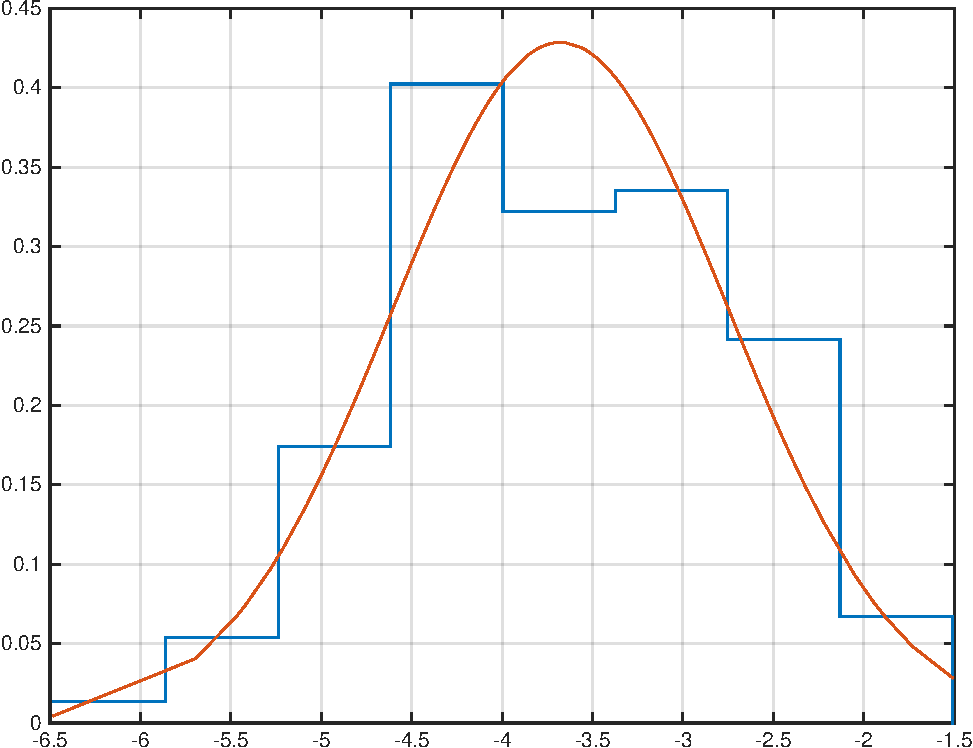
\includegraphics[width=0.7\textwidth]{graphic-1.pdf}
    \caption{Гистограмма и график функции плотности распределения нормальной случайной величины.}
\end{figure}



\newpage
\subsection{График эмпирической функции распределения и функции распределения нормальной случайной величины с математическим ожиданием $\hat{\mu}$ и дисперсией $S^2$}

\begin{figure}[h]
    \centering
    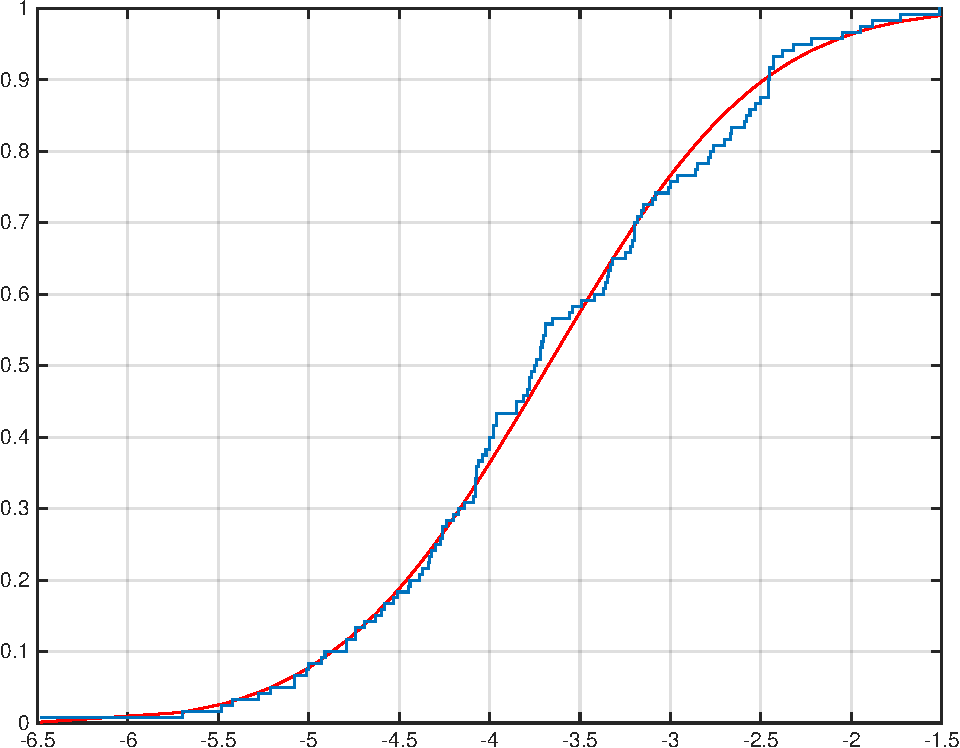
\includegraphics[width=0.7\textwidth]{graphic-2.pdf}
    \caption{График эмпирической функции распределения и функции распределения нормальной случайной величины.}
\end{figure}